\documentclass[a4paper, 12pt]{article}
\usepackage[utf8x]{inputenc}
\usepackage{cmap}
\usepackage[english, russian]{babel}
\usepackage{indentfirst}
\usepackage[left=20mm, top=20mm, right=20mm, bottom=20mm]{geometry}
\usepackage{tikz}
\usepackage{float}
\usepackage{amsmath, amsfonts, amssymb}
\usepackage{graphicx}
\usepackage{fancybox, fancyhdr}
\usepackage{hyperref}
\usepackage{listings}
\usepackage{caption}
\usepackage{subcaption}
\usepackage{xcolor}
\usepackage{attachfile2}
\pagestyle{fancy}
\fancyhf{}
\fancyhead[L]{Лабораторная работа №1}
\fancyhead[R]{ЛСАУ}
\fancyfoot[C]{\thepage}
\graphicspath{{images/}}
\usetikzlibrary{patterns}
\definecolor{LightGray}{gray}{0.95}
\definecolor{LightGray2}{gray}{0.7}
\lstdefinestyle{code}{
    language=Python, % replace with needed language
    basicstyle=\footnotesize\ttfamily,
    backgroundcolor=\color{LightGray},
    showspaces=false,
    showstringspaces=false,
    showtabs=false,
    tabsize=4,
    captionpos=b,
    breaklines=true,
    breakatwhitespace=false,
    frame=single,
    rulecolor=\color{LightGray2},
    linewidth=\linewidth,
    keywordstyle=\color{blue}\bfseries,
    commentstyle=\color{green!40!black},
    stringstyle=\color{purple},
    escapeinside={\%*}{*)},
    inputencoding=utf8x,
    xleftmargin=0pt,
    framexleftmargin=0pt,
    framexrightmargin=0pt
}
\lstset{style=code}
\hypersetup{
    colorlinks=true,
    linkcolor=blue,
    filecolor=magenta,
    urlcolor=cyan,
    pdftitle={contents setup},
    pdfpagemode=FullScreen,
}
\setlength{\parskip}{1.5mm}
\setlength{\headheight}{15pt}
\setlength{\footskip}{15pt}
\allowdisplaybreaks
\DeclareMathOperator{\sinc}{sinc}
\newcommand{\frc}[2]{\raisebox{2pt}{$#1$}\big/\raisebox{-3pt}{$#2$}}

\begin{document}
    \begin{titlepage}
        \begin{center}
            
\includegraphics[width=0.3\textwidth]{itmo.png}
        \vfill

        Федеральное государственное автономное образовательное учреждение высшего образования
        «Национальный Исследовательский Университет ИТМО»\\

        \vfill
        {\large\bf ЛАБОРАТОРНАЯ РАБОТА №1}\\
        {\large\bf ПРЕДМЕТ «ЛСАУ»}\\
        {\large\bf ТЕМА «КАНОНИЧЕСКИЕ ФОРМЫ ПРЕДСТАВЛЕНИЯ
        ДИНАМИЧЕСКИХ СИСТЕМ»}\\
        {\large\bfВариант 7}\\
        \vfill

        \begin{flushright}
            \begin{minipage}{.45\textwidth}
            {
                \hbox{Преподаватель: Золотаревич В. П.}
                \hbox{Студент: Чебаненко Д. А.}
                \hbox{Поток:ЛСАУ 4.1.1}
                \hbox{}
                \hbox{Факультет: СУиР}
                \hbox{Группа: R3341}
            }
            \end{minipage}
        \end{flushright}

        \vfill

        Санкт-Петербург\\
        2024
        \end{center}
    \end{titlepage}

    \tableofcontents

    \newpage
    \section{Задание 1}
        \noindent В начале составим дифференциальное уравнение по входным параметрам.
        $$y''+3y' + 7y = 6u' + 10u$$
        Переведем уравнение к операторной форме
        $$p^2y = p6u - p3y + 10u - 7y$$
        Выразим входной сигнал
        $$y = \frac{1}{p} (6u - 3y) + \frac{1}{p^2}(10u-7y)$$
        Далее построим схему в simulink
        \begin{figure}[H]
            \centering
            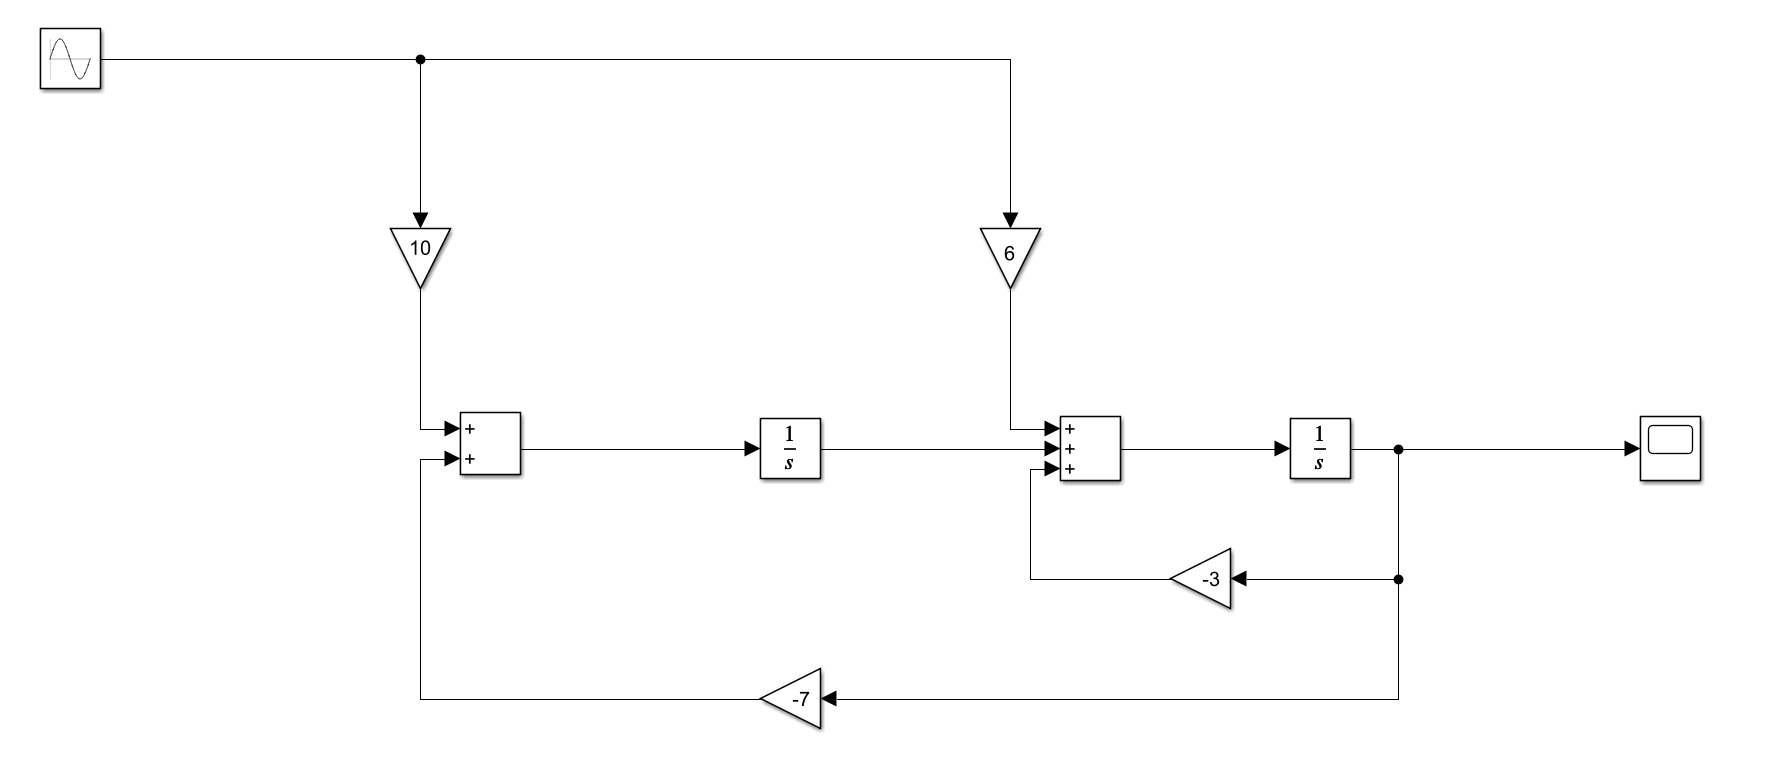
\includegraphics[scale=0.4]{sim.png}
            \captionsetup{skip=0pt}
            \caption{Схема в simulink}
            \label{fig:1imspdf}
        \end{figure}
        Выведем график функции Хевисайда
        \begin{figure}[H]
            \centering
            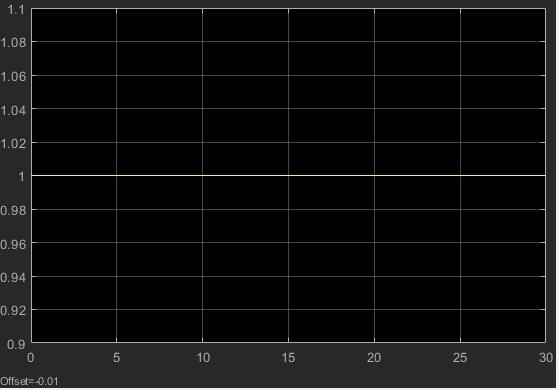
\includegraphics[scale=0.4]{hev.jpg}
            \captionsetup{skip=0pt}
            \caption{Функция Хевисайда 1(t)}
            \label{fig:2imspdf}
        \end{figure}\newpage
        Подадим на вход функцию Хевисайда $1(t)$
        \begin{figure}[H]
            \centering
            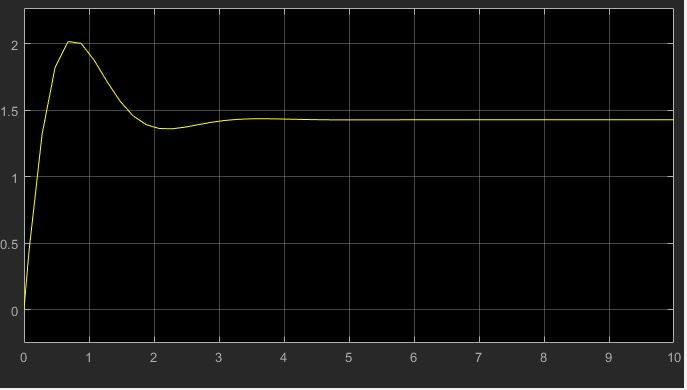
\includegraphics[scale=0.4]{hev1.jpg}
            \captionsetup{skip=0pt}
            \caption{Реакция системы на функцию Хевисайда 1(t)}
            \label{fig:2imspdf}
        \end{figure}
        Теперь подадим на вход $2\sin(t)$
        \begin{figure}[H]
            \centering
            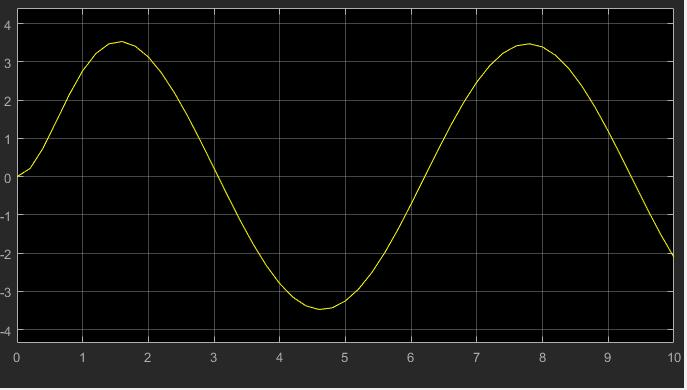
\includegraphics[scale=0.4]{2sin(t).jpg}
            \captionsetup{skip=0pt}
            \caption{Реакция системы на функцию $2\sin(t)$}
            \label{fig:3imspdf}
        \end{figure}
        \noindent Рассчитаем начальные условия при $y(0) = 1\text{ и } y'(0) = 0.4$\\
        $$y(0) = z_1(0) = 1$$
        $$z_2(0) = y'(0) + 6u + 3y = 3.4$$
        Запустим систему при нулевом входе и c рассчитанными начальными условиями.
        \begin{figure}[H]
            \centering
            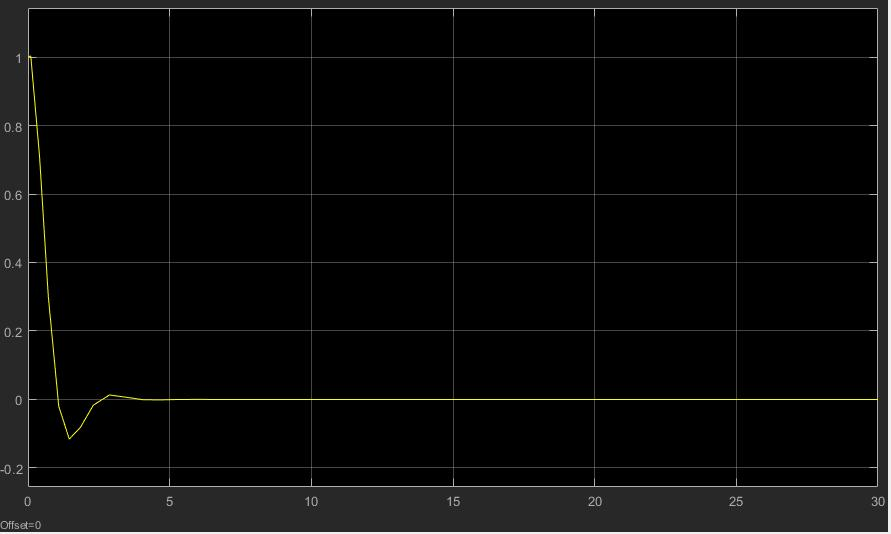
\includegraphics[scale=0.37]{1.3.jpg}
            \captionsetup{skip=0pt}
            \caption{Вид системы при $u = 0$}
            \label{fig:4imspdf}
        \end{figure}
        \section{Задание 2}
        Составим систему соответствующую варианту.
        $$\begin{cases}
            x_1' = -3x_1 + u\\
            x_2' = 2x_1 + x_3\\
            x_3' = x_1 -6x_2 - x_3 + u\\
            y = 0.5x_1+ 2.5x_2
         \end{cases}$$
         Построим схему соответствующую данной системе.
         \begin{figure}[H]
            \centering
            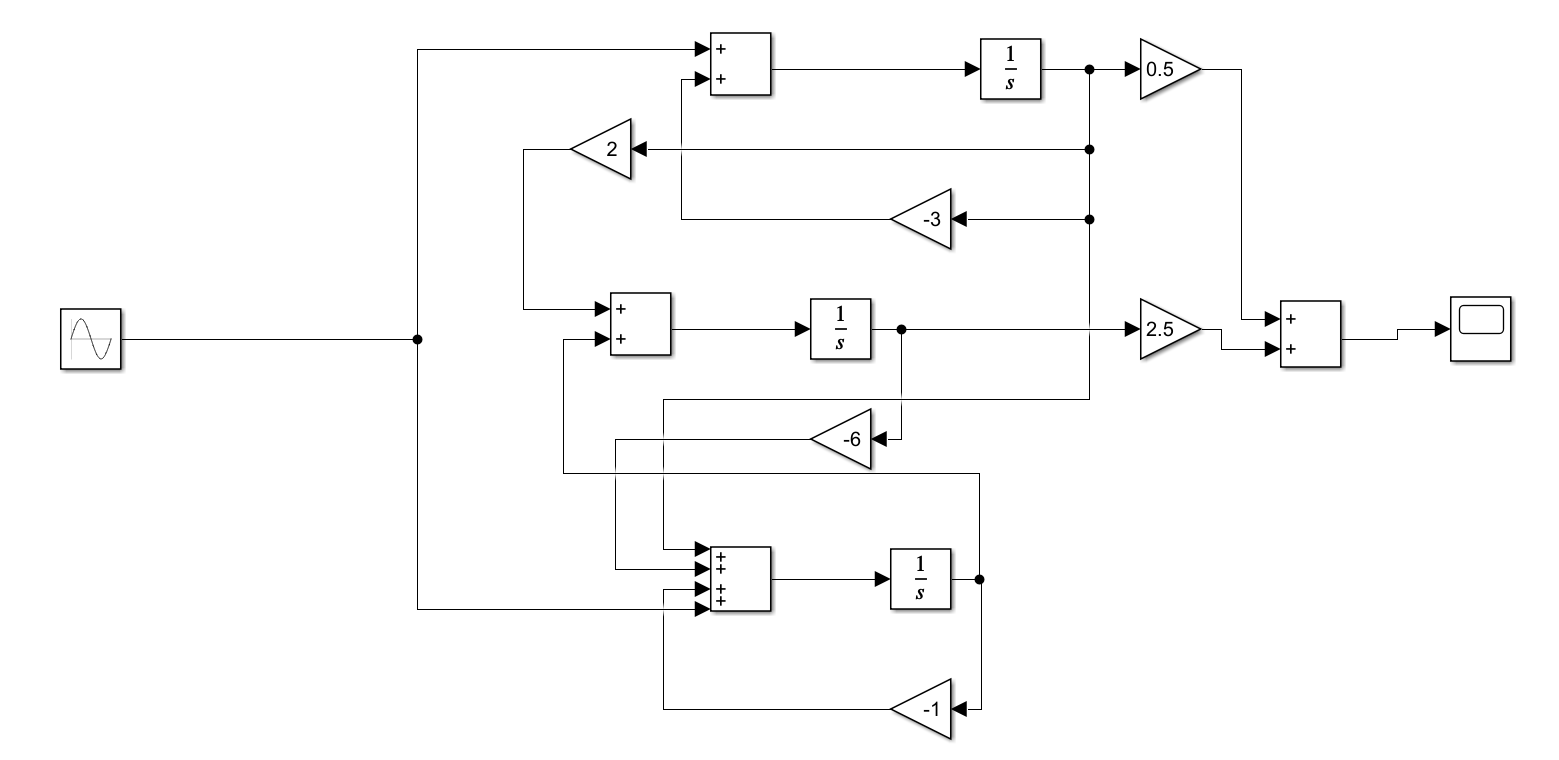
\includegraphics[scale=0.4]{2.0.png}
            \captionsetup{skip=0pt}
            \caption{Схема системы}
            \label{fig:5imspdf}
        \end{figure}
        Подадим на вход функцию Хевисайда
        \begin{figure}[H]
            \centering
            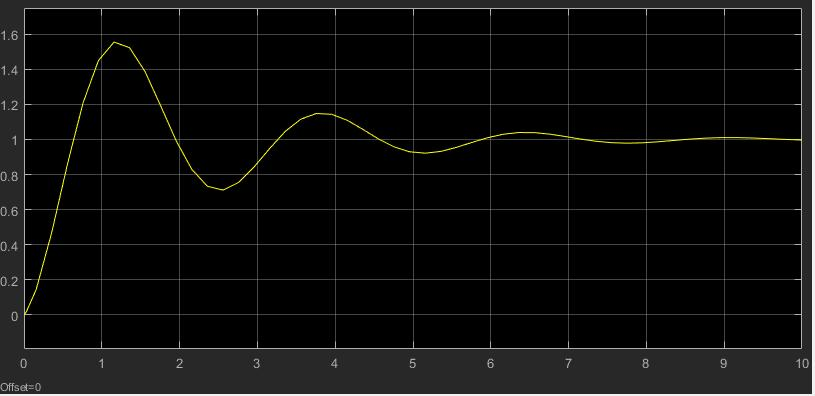
\includegraphics[scale=0.4]{2.1.jpg}
            \captionsetup{skip=0pt}
            \caption{Реакция системы на единичный скачек}
            \label{fig:5imspdf}
        \end{figure}
        \newpage
        Подадим на вход $2\sin(t)$
        \begin{figure}[H]
            \centering
            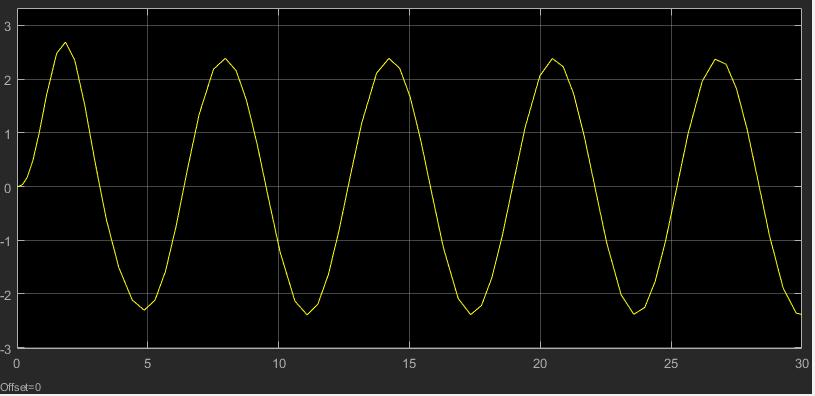
\includegraphics[scale=0.4]{2.2.jpg}
            \captionsetup{skip=0pt}
            \caption{Реакция системы на $2\sin(t)$}
            \label{fig:5imspdf}
        \end{figure}
        Запустим систему при $u = 0$ и параметрами рассчитанными исходя из варианта.
        \begin{figure}[H]
            \centering
            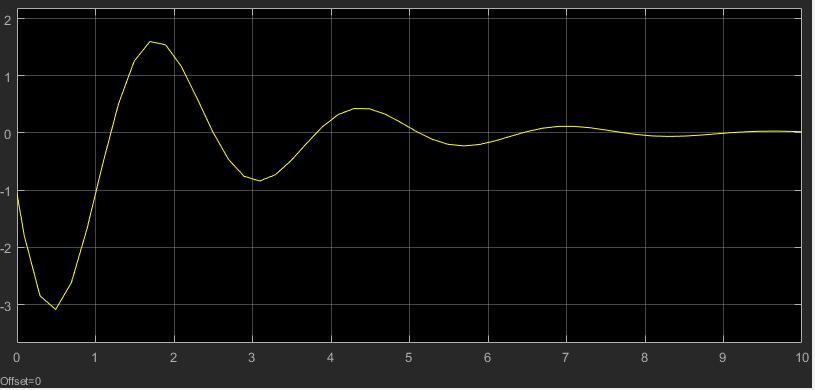
\includegraphics[scale=0.4]{2.3.jpg}
            \captionsetup{skip=0pt}
            \caption{Система при $u = 0$}
            \label{fig:5imspdf}
        \end{figure}
        \section{Вывод}
\end{document}
